%!TEX root = nonabelions.tex

\chapter{Statistical repulsion}\label{chap:statistical repulsion}

In this chapter we give a lower bound for the kinetic energy of free anyons. This gives rise to what is known as statistical repulsion, an essentially geometric effect of the exchange operator that causes an effective repulsion of indistinguishable particles. This has consequences for the density of the wave function, and might thus be measured. This chapter is in part based on \cite{methmmp,lundholm-solovej,mancarella}. See also \cite{larson-lundholm} for the case of what is known as extended abelian anyons.


A quantum system is generally determined by a Hamiltonian $\hat{H} = \hat{T} + \hat{V}$ where $\hat{T} = \hat{p}⋅\hat{p} = -∇²$ is the kinetic energy operator, $\hat{p} = -i∇$ is the momentum operator, and $\hat{V}$ is the potential energy operator. We shall consider free particles, i.e.\ $\hat{V} = 0.$






\section{Fermionic statistical repulsion}

Recall that the exchange operator is the braid group representation of a simple exchange of particles. In the case of bosons and fermions in $d ≥ 3$ dimensions the exchange operator is simply the identity and $-1$, respectively. That is,
\begin{equation}
  ψ(x_2, x₁) = \pm ψ(x₁, x_2).
\end{equation}
For fermions, this leads to the well-known Pauli exclusion principle. Simply stated, if $x₁ = x_2$ it immediately follows that $ψ(x₁, x₁) = 0$, the particles cannot occupy the same position. More generally, the anti-symmetry of the fermionic wave function causes the kinetic energy to increase as the particles tend closer to each other. This is an effective repulsion due to the particle statistics. We shall now see this in more detail.

Consider $n$ indistinguishable particles on $ℝᵈ$. Let $x₁, …, x_n$ be the coordinates of the particles, i.e.\ $xⱼ ∈ ℝᵈ$. This collection of particles is described by an $n$-particle wave function $ψ(x₁, …, x_n) ∈ L^2(ℝ^{dn})$, i.e.\ a square integrable complex-valued function on $ℝ^{dn}$. The kinetic energy $T$ of this system is defined as
\begin{equation}
  T ≔ ⟨ψ|\hat{T}|ψ⟩ = ∑_{j=1}^n ∫_{ℝ^{dn}} |∇ⱼ ψ|^2 dx.
\end{equation}
In the present discussion we shall assume that $ψ$ is normalized and in the domain of the operator. A detailed discussion for abelian anyons can be found in \cite{larson-lundholm} and \cite{lundholm-solovejAHP}, see also \cite{dellantonio}.

Let the particles be fermions, i.e.\ $ψ ∈ L_\text{asym}^2(ℝ^{dn})$. This is the subspace of functions $ψ$ in $L^2(ℝ^{dn})$ such that $ψ(…, xⱼ, …, xₖ, …) = - ψ(…, xₖ, …, xⱼ, …)$ for $j \ne k$. In this case, we have the following theorem \cite{hoholt,methmmp}.

\begin{theorem}[Many-body Hardy inequality for fermions]\label{thm:hardy fermion}
  In the described setting with $ψ$ being an $n$-particle fermionic wave function, the following lower bound for the kinetic energy holds
  \begin{equation}\label{eq:fermion ineq}
    ∫_{ℝ^{dn}} ∑_{j=1}^n |∇ⱼψ|^2 dx \ge
    \frac{d²}{n} ∫_{ℝ^{dn}} ∑_{1≤j<k≤n} \frac{|ψ|^2}{|xⱼ-xₖ|^2} dx +
    \frac{1}{n} ∫_{ℝ^{dn}} \left|∑_{j=1}^n ∇ⱼ ψ \right|^2 dx.
  \end{equation}
\end{theorem}

The first integral shows that fermionic particles have an inverse-squared pairwise effective repulsion. The second integral on the right-hand side essentially gives the contribution of the motion of the center of mass.

We give an outline of the proof.

\begin{proof}
  First, one can show
  \begin{equation}
    ∑_{j=1}^n |∇ⱼ ψ|^2 = \frac{1}{n} ∑_{1 \le j < k \le n} \left| (∇ⱼ - ∇ₖ) ψ \right|^2 + \frac{1}{n} \left| ∑_{j=1}^n ∇ⱼ ψ \right|²,
  \end{equation}
  by expanding the expression, known as the many-body parallelogram identity. The last term sum to the center of mass motion and is not of interest. We focus on the first sum on the right-hand side.

  Introduce relative coordinates for each pair $(j,k)$ of particles,
  \begin{equation}
    \begin{aligned}
      x_{jk}^\text{rel} &≔ (xⱼ - xₖ)/2, & x_{jk}^\text{cm} &≔ (xⱼ + xₖ)/2, \\
      ∇_{x_{jk}^\text{rel}} &≔ ∇ⱼ - ∇ₖ, & ∇_{x_{jk}^\text{cm}} &≔ ∇ⱼ + ∇ₖ.
    \end{aligned}
  \end{equation}
  It shall be useful to split the coordinates as $x = (xⱼ, xₖ; x')$ where $x' ∈ ℝ^{d(n-2)}$ and $j < k$ fixed. Next, define the relative wave function
  \begin{equation}
    u(x_{jk}^\text{rel}, x_{jk}^\text{cm}) ≔ ψ(x₁, …, xⱼ=x_{jk}^\text{cm}+x_{jk}^\text{rel}, …, xₖ = x_{jk}^\text{cm}-x_{jk}^\text{rel}, …, x_n).
  \end{equation}
  We then have $u(-x_{jk}^\text{rel}, x_{jk}^\text{cm}) = -u(x_{jk}^\text{rel}, x_{jk}^\text{cm})$ for fermions, by the anti-symmetry of $ψ$.

  With this change of variables we have
  \begin{equation}
    \begin{aligned}
      ∫_{ℝ^{dn}} \left|(∇ⱼ-∇ₖ)ψ\right|^2 dx
      &= ∫_{ℝ^{d(n-2)}} ∫_{ℝᵈ \times ℝᵈ} \left|(∇ⱼ-∇ₖ)ψ\right|^2 dxⱼdxₖdx' \\
      &= ∫_{ℝ^{d(n-2)}} ∫_{ℝᵈ \times ℝᵈ} \left|∇_{x_{jk}^\text{rel}}u\right|^2  2 dx_{jk}^\text{rel}dx_{jk}^\text{cm} dx'.
    \end{aligned}
  \end{equation}

  Finally, one shows, for anti-symmetric (fermionic) wave functions,
  \begin{equation}
    ∫_{ℝᵈ} \left|∇_{x_{jk}^\text{rel}} u \right|^2 dx_{jk}^\text{rel} \ge \frac{d^2}{4} ∫_{ℝᵈ} \frac{|u|^2}{|x_{jk}^\text{rel}|^2} dx_{jk}^\text{rel}
  \end{equation}
  from which the result follows.
\end{proof}

In the outline of the proof we skipped the details of the last step. To obtain a similar inequality for anyons, it is exactly this step that shall be important, and we now look into this in more detail in the case $d = 2$.














\section{Anyonic statistical repulsion}

In the proof outline of \cref{thm:hardy fermion}, the assumption that $ψ$ is anti-symmetric is used only in the last step where the expression
\begin{equation}
  ∫_{ℝᵈ} \left|∇_{x_{jk}^\text{rel}} u(x) \right|^2 dx_{jk}^\text{rel}
\end{equation}
is considered. We now extend this to the more general case with
\begin{equation}\label{eq:rel boundary cond}
  u(-x_{jk}^\text{rel}, x_{jk}^\text{cm}) = U_γ u(x_{jk}^\text{rel}, x_{jk}^\text{cm})
\end{equation}
for general anyons with simple exchange represented by $U_γ$. This implicitly assumes $d = 2$ so that $U_γ$ determines braid statistics. Generally, $U_γ$ may denote simple exchange around a number of inner anyons, i.e.\ $γ$ denotes a loop in configuration space, enclosing a number of fixed anyons. We shall return to the details of this later.

In polar coordinates $x_{jk}^\text{rel} = (r, φ)$ we have
\begin{equation}
  ∫_{ℝ²} \left|∇_{x_{jk}^\text{rel}} u \right|^2 dx_{jk}^\text{rel} =
  ∫_{r=0}^∞ ∫_{φ=0}^{2π} \left( \left|∂ᵣu\right|^2 + \frac{\left|∂_φu\right|²}{r²} \right) r dφ dr.
\end{equation}
It is the angular derivative term that gives the contribution of the exchange statistics. Thus, we only consider this integral
\begin{equation}
  ∫₀^{2π} \left|∂_φu\right|² dφ.
\end{equation}
Since we consider $r$ fixed, we define $u(φ) ≔ u(r,φ)$. In this way, the loop $γ = γᵣ$ is determined by $r$ and the number of encircled fixed anyons varies with $r$. Loops with different number of encircled fixed anyons are not homotopically equivalent and thus the exchange operator $U_{γᵣ}$ depends on $r$. The boundary condition \cref{eq:rel boundary cond} may thus be written as $u(π) = U_{γᵣ} u(0)$. Furthermore,
\begin{equation}
  \begin{aligned}
    ∫₀^{2π} \left|∂_φu\right|² dφ
    &=
    ∫₀^π \left|∂_φu(φ)\right|² dφ +
    ∫₀^π \left|∂_φu(π+φ)\right|² dφ \\
    &=
    ∫₀^π \left|∂_φu(φ)\right|² dφ +
    ∫₀^π \left|∂_φU_{γᵣ}u(φ)\right|² dφ \\
    &=
    2∫₀^π \left|∂_φu\right|² dφ
  \end{aligned}
\end{equation}
since unitary operators are norm preserving.

Define the operator
\begin{equation}\label{eq:D}
  D = -i∂_φ, \quad \operatorname{Dom}D = \{u : u, ∂_φ u ∈ L²([0,π]), u(π) = U_{γᵣ}u(0)\}.
\end{equation}
The expectation value of $D²$ with $\operatorname{dom} D² = \{ u : u, Du ∈ \operatorname{dom}D \}$,
\begin{equation}
  \begin{aligned}
    ⟨u|D²|u⟩
    &= -∫₀^π \overline{u} ∂_φ² u \,dφ \\
    &= -\overline{u}∂_φu\Big|₀^π + ∫₀^π ∂_φ\overline{u} ∂_φ u \,dφ \\
    &= ∫₀^π ∂_φ\overline{u} ∂_φ u \,dφ \\
    &= ∫₀^π |∂_φu|² dφ
  \end{aligned}
\end{equation}
is precisely the integral we are considering. In the above calculation, the boundary term vanishes since $U_{γᵣ}$ is unitary,
\begin{equation}
  \begin{aligned}
    \overline{u}∂_φu\Big|₀^π
    &= \overline{u}(π)∂_φu(π) - \overline{u}(0)∂_φu(0) \\
    &= U_{γᵣ}^*\overline{u}(0)U_{γᵣ}∂_φu(0) - \overline{u}(0)∂_φu(0) \\
    &= (U_{γᵣ}^*U_{γᵣ} - I)\overline{u}(0)∂_φu(0) \\
    &= 0.
  \end{aligned}
\end{equation}
Similarly, one shows that $D$ is self-adjoint. Thus, also $D²$ is self-adjoint, so the Rayleigh quotient of $D²$ can be used to obtain a lower bound by the min-max theorem,
\begin{equation}
  ∫₀^π |∂_φu|² dφ = ⟨u|D²|u⟩ ≥ \inf σ(D²) ≕ λ_{0,γᵣ}²,
\end{equation}
where we assume that $u$ is normalized in $L²[0,π]$.

By the spectral theorem we have
\begin{equation}
  σ(D²) = \{λ² : λ ∈ σ(D)\}
\end{equation}
The spectrum of $D$ is straight forward to compute.

\begin{lemma}
  The spectrum of $D$ is given by
  \begin{equation}
    σ(D) = \{ λ : e^{iλπ} \text{ is an eigenvalue of $U_{γᵣ}$} \}
  \end{equation}
\end{lemma}
\begin{proof}
  The eigenequation for $D$ gives
  \begin{equation}
    Du = λu ⟺ -iu' = λu ⟺ u(φ) = C e^{iλφ}
  \end{equation}
  for a non-zero constant vector $C ∈ ℂᵏ$. Moreover, the boundary condition \cref{eq:D} implies
  \begin{equation}
    u(π) = U_{γᵣ} u(0) ⟹ Ce^{iλπ} = U_{γᵣ}C,
  \end{equation}
  i.e.\ $e^{iλπ}$ is an eigenvalue of $U_{γᵣ}$, with eigenvector $C$.
\end{proof}

Thus, we have a lower bound for the angular term, carrying the contribution of the anyonic statistics leading to statistical repulsion.

\begin{theorem}\label{thm:inf spec bound}
  Anyons with exchange operator $U_{γᵣ}$ satisfy the inequality
  \begin{equation}
    ∫₀^π |∂_φu|² dφ ≥ \inf \, \{ λ² : e^{iλπ} \text{ is an eigenvalue of $U_{γᵣ}$} \} = λ_{0,γᵣ}².
  \end{equation}
\end{theorem}

\begin{remark}
  Each eigenvalue of $U_{γᵣ}$ is on the form $e^{iαπ}$ with $0≤α<2$ since $U_{γᵣ}$ is unitary. By the theorem, each eigenvalue gives rise to a family of possible energy levels
  \begin{equation}
    \{ (α+2q)² : q ∈ ℤ \}
  \end{equation}
  for the angular Hamiltonian $H = D²$, with corresponding eigenfunctions
  \begin{equation}
    u_q(φ) = C₁e^{i(α+2q)φ}.\qedhere
  \end{equation}
\end{remark}


\begin{remark}
  Instead of introducing anyonic exchange as the condition $u(π) = U_{γᵣ} u(0)$ one can use the framework of fiber bundles to model anyons by changing the kinetic energy operator from
  \begin{flalign}
    &\text{\textit{Anyon gauge:}} & \widehat{T} &= ∑_{j=1}^n -∇ⱼ^2 &
  \intertext{to}
    &\text{\textit{Magnetic gauge:}} & \widehat{T}_A &= ∑_{j=1}^n \left( -i ∇ⱼ + Aⱼ \right)^2,&
  \end{flalign}
  where $A$ is a connection one-form on the bundle of which the wave function is a section. In this way the wave function may be chosen periodic $u(π)=u(0)$, i.e.\ the anyonic exchange is then completely captured by $Aⱼ$ and $ψ$ is bosonic \cite{nakahara}.
  % TODO: The following example illustrates this.
  % \begin{example}
  %   Skriv ner fr. tidigare anteckningar: Två abelska anyoner. Connection $Aⱼ = α ∑_{j≠k} \frac{(xⱼ-xₖ)^⟂}{|xⱼ-xₖ|²}$.
  % \end{example}
\end{remark}
















\section{Separating the state space}

In the above discussion, the exchange operator $U_{γᵣ}$ is defined to be a simple exchange of the pair $(xⱼ,xₖ)$, possibly around $p$ other anyons. We started by considering the expression
\begin{equation}
  ∫_{ℝ^{2(n-2)}} ∫_{ℝ² \times ℝ²} \left|∇_{x_{jk}^\text{rel}}u\right|^2  2 dx_{jk}^\text{rel}dx_{jk}^\text{cm} dx'.
\end{equation}
The inner integral concerns anyons $j$ and $k$ with the remaining $n-2$ considered fixed. The inner integral is rewritten as
\begin{equation}
  \begin{aligned}
    ∫_{ℝ²} \left|∇_{x_{jk}^\text{rel}} u \right|^2 dx_{jk}^\text{rel}
    &= ∫_{r=0}^∞ ∫_{φ=0}^{2π} \left( \left|∂ᵣu\right|^2 + \frac{\left|∂_φu\right|²}{r²} \right) r dφ dr \\
    &≥ ∫_{r=0}^∞ ∫_{φ=0}^{2π} \left( \left|∂ᵣu\right|^2 + λ_{0,γᵣ}²\frac{\left|u\right|²}{r²} \right) r dφ dr
  \end{aligned}
\end{equation}
and we assume $u$ satisfies the anyonic boundary condition $u(π) = U_{γᵣ} u(0)$. The exchange operator $U_{γᵣ}$ may depend on $r$ since the number of encircled anyons in the loop $γᵣ$ may affect the exchange operator $U_{γᵣ}$. To make this precise we separate the state space into open annuli (regions between two concentric circles) centered at $x_{jk}^\text{cm}$, such that none of the fixed $n-2$ anyons are at the interior of an annulus, cf.\ \cref{fig:annuli}. This gives a separation of $ℝ^2$ into regions with increasing number $p$ of the $n-2$ fixed anyons. Let $r₁ \le r₂ \le … \le r_{n-2}$ be the radial coordinate of the $n-2$ fixed anyons. The innermost annulus is an open disk (degenerate annulus) with radius $r₁$, the second innermost annulus is the region between circles of radius $r₁$ and $r_2$, etc. Note that the circles with radii $r₁, r₂, …, r_{n-2}$ are not contained in any annuli, since the anyons cannot pass through each other, and we are considering angular motion. If the radii of two fixed anyons coincide, then there is no annulus separating them. The removal of these circles removes more points than $\bbDelta$, however this is no issue since the circles of radius $rⱼ$ have measure zero.

In this way, exchange of particles $j$ and $k$ depend on $r$, i.e.\ $U_{γᵣ} = U_{γᵣ}(r)$. Since the dependence on $r$ is exclusively due to the $p$ number of encircled fixed anyons, we introduce the notation
\begin{equation}
  Uₚ ≔ U_{γᵣ}(r), \quad r_{p-1} < r < rₚ,
\end{equation}
with $r₀ = 0$ and $r_{n-1} = ∞$. This is precisely the exchange braid introduced in \cref{def:exchange braid}. The exchange corresponding to $Uₚ$ is visualized in \cref{fig:Up exchange}.

\begin{figure}[h]
  \centering
  \begin{tikzpicture}[scale=0.8]
    \draw[->] (-3.75,0) -- (3.75,0) node[below] {$x$};
    \draw[->] (0,-3.75) -- (0,3.75) node[right] {$y$};
    \draw (0,0) circle (1.25);
    \draw (0,0) circle (2);
    \draw (0,0) circle (3);
    \node at (0.55, 0.35) {$p = 0$};
    \node at (0.55, 1.5) {$p = 1$};
    \node at (0.55, 2.375) {$p = 2$};
    \node at (0.55, 3.25) {$p = 3$};
    \node at ({1.25*cos(220)}, {1.25*sin(220)}) {$\bullet$};
    \node at ({2*cos(130)}, {2*sin(130)}) {$\bullet$};
    \node at ({3*cos(-55)}, {3*sin(-55)}) {$\bullet$};
    \node at (1.5, -0.2) {$r₁$};
    \node at (2.25, -0.2) {$r_2$};
    \node at (3.25, -0.2) {$r_3$};
  \end{tikzpicture}
  \caption{Illustration of annuli separating $ℝ^2$ into regions with increasing number $p$ of contained anyons. A blob $\bullet$ denotes a fixed anyon. In each annulus, exchange of the two free anyons, i.e.\ as $φ$ increases from $0$ to $π$, a given number $p$ of fixed anyons will be encircled.}
  \label{fig:annuli}
\end{figure}

\begin{figure}[h]
  \centering
  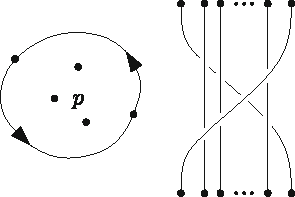
\includegraphics{img/interchange_loop_p.pdf}
  \caption{Exchange of a pair of anyons around $p$ fixed anyons. Figure taken from \cite{lundholm-solovej}.}
  \label{fig:Up exchange}
\end{figure}








\subsection{Abelian anyons}\label{sec:statistical repulsion abelian ayons}

Abelian anyons have an exchange operator on the form $U₀ = e^{iαπ}$ for $0≤α<2π$. Moreover, by \cref{res:abelian repr} every simple exchange is determined by the same representation. Thus,
\begin{equation}
  Uₚ = ρ(σ₁)ρ(σ₂)⋯ρ(σₚ)ρ(σ_{p+1})ρ(σₚ)⋯ρ(σ₂)ρ(σ₁) = e^{i(2p+1)απ}.
\end{equation}
In this case, the spectrum for $D²$ is given by
\begin{equation}
  σ(D²) = \{ \left( (2p+1)α + 2q \right)² : q ∈ ℤ \}
\end{equation}
and thus \cref{thm:inf spec bound} yields the following result for $n → ∞$.

\begin{theorem}
  Abelian anyons with exchange operator $U₀ = e^{iαπ}$ satisfy the lower bound
  \begin{equation}
    \begin{gathered}
      ∫₀^π |∂_φu|² dφ ≥ λ_{0,γᵣ}² = \\
      % \inf_{p,q ∈ ℤ} \left( (1+2p)α + 2q \right)² = \\
      = \begin{cases}
        \frac{1}{ν^2}, & \text{if $α = \frac{μ}{ν}$ with $μ ∈ ℤ, ν ∈ ℕ₊$ relatively prime and $μ$ odd}, \\
        0, & \text{otherwise}
      \end{cases}
    \end{gathered}
  \end{equation}
\end{theorem}

The last equality in the theorem is essentially a number-theoretic result, proved in proposition 5 in \cite{lundholm-solovej}.

From this we have an immediate corollary for bosons ($α = 0$) and fermions ($α = 1$).

\begin{corollary}
  With $α = 0$, the exchange operator is
  \begin{equation}
    U_p = e^{i(1+2p)απ} = 1
  \end{equation}
  for all $p$, i.e.\ bosons do not ``see'' each other, and they have no statistical repulsion; $\inf σ(D²) = 0$.

  With $α = 1$, the exchange operator is
  \begin{equation}
    U_p = e^{i(2p+1)απ} = -1
  \end{equation}
  for all $p$, i.e.\ fermions do not ``see'' the encircled $p$ fermions. However, the particles in the exchange pair do ``see'' each other, in the sense that their wave function changes sign after they have been exchanged, as expected. This gives a non-zero statistical repulsion, $\inf σ(D²) = λ_{0,γᵣ}² = 1$ for all $γᵣ$.
\end{corollary}

The effects of the statistical repulsion may have consequences for the wave function density, e.g. the wave function may be forced to vanish on $\bbDelta$; as particles get close to each other. As we have discussed, the density may be measured. Thus, understanding the effects of the statistical repulsion may help in the experimental search for anyons. It may also affect the free energy and the stability of anyonic many-body systems, see \cite{lundholm-solovej,many-anyon trial states,lundholm-solovejAHP}.






\subsection{Non-abelian anyons}

The exchange operator $Uₚ$ of non-abelian anyons cannot be characterized in a straight forward way as for abelian anyons, essentially due to $ρ(σⱼ)$ and $ρ(σ_{j+1})$ not commuting. Because of this, determining the spectrum $σ(Uₚ)$ and thus the lower bound
\begin{equation}
    ∫₀^π |∂_φu|² dφ ≥ λ_{0,γᵣ}² = \inf \, \{ λ² : e^{iλπ} ∈ σ(Uₚ) \},
\end{equation}
becomes problematic. In light of this, we must better understand how the non-abelian exchange operator $Uₚ$ arises. To do this, we introduce the general framework of abstract anyon models in the following chapter. First we make the following general observation.

\begin{remark}
  The abelian part of $U ∈ U(k)$, i.e.\ the $U(1)$ part in the factorization $U(k) = U(1) × SU(k)$, is given by $e^{iθ}$ such that
  \begin{equation}
    U = e^{iθ} U₀
  \end{equation}
  where $\det U₀ = 1$. Note the relation
  \begin{equation}
    \det U = \det(e^{iθ}U_0) = e^{ikθ}.
  \end{equation}
  Varying the abelian phase $θ$ can be seen as shifting the eigenvalues of $U$ uniformly along the complex unit circle. In particular, with $U₀$ diagonalized as $U₀ = \operatorname{diag}(e^{iθ₁}, …, e^{iθₖ})$, changing the abelian phase according to $e^{iθ} ↦ e^{-iθⱼ}$ gives $U$ a zero eigenvalue. Thus, implying zero statistical repulsion. However, the abelian part can generally not be decoupled and controlled independently.
\end{remark}
